\chapter{Vista de casos de uso}
\section{Introducci\'on}
En esta vista nos disponemos a detallar varios casos de uso que pertenecen al sistema. Estos casos de uso son simplemente una descripci\'on del comportamiento del sistema tal y como lo ver\'ian todos los usuarios participantes.

\section{Actores}
El sistema lo compone los siguientes usuarios:
\begin{description}
\item[Administrador] Este tipo de usuario es el encargado de crear/inicializar/eliminar los distintos entornos EHC y dispositivos.
\item[Super usuario] Este usuario es introducido en una configuraci\'on inicial por el administrador. El control en su entorno EHC es total, y tambi\'en tiene el suficiente poder para crear distintos tipos de usuarios para los participantes del sistema con unos privilegios determinados por el super usuario. 
\item[Usuario] Es un tipo de usuario creado por el super usuario. Su funcionalidad depende de los privilegios otorgados por el super usuario que ha creado este usuario, que puede ser desde un simple usuario con funciones de consulta hasta un usuario que pueda manipular y controlas los dispositivos del entorno EHC.
\end{description}

A trav\'es de la figura ~\ref{fig:actores} mostramos un esquema general de la organizaci\'on de los usuarios en el sistema:

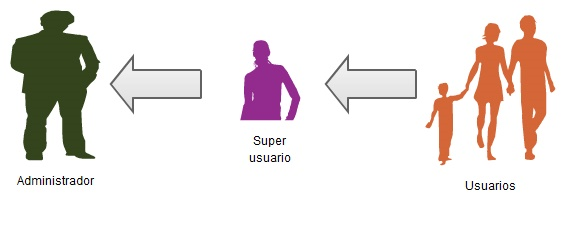
\includegraphics[width=0.7\textwidth]{4.Disenio/Imagenes/Actores}


\section{Casos de uso}
\subsection{Visi\'on general de los casos de uso}
En este diagrama se representan las funcionalidades y comportamientos del sistema dependiendo del tipo de usuario que se encuentre en el entorno. Gracias al an\'alisis de estos casos de uso, hemos obtenido los requisitos funcionales y no funcionales del sistema de una forma en la que as\'i se agiliza el proceso de an\'alisis del sistema.
 
Mostramos a trav\'es de las figuras ~\ref{fig:cuSuperusuario} y ~\ref{fig:cuSuperusuario} los diagrama de casos de uso tanto del super usuario como del administrador. Evitamos incluir el diagrama del usuario b\'asico ya que el super usuario es una extensi\'on de este.

\begin{figure}[h!]
	\centering
	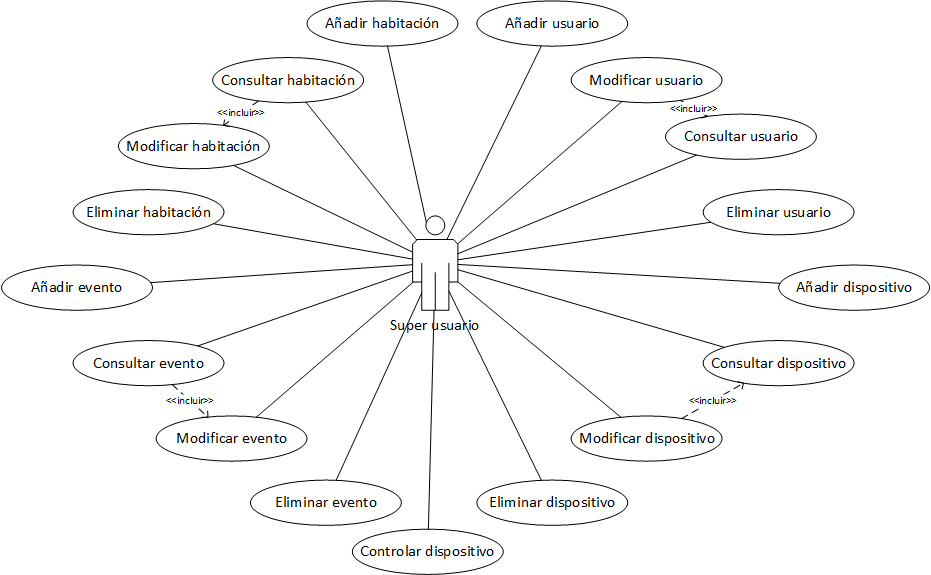
\includegraphics[width=0.7\textwidth]{4.Disenio/Imagenes/CU-Superusuario}
	\caption{Casos de uso del super usuario.}
	\label{fig:cuSuperusuario}
\end{figure}

\begin{figure}[h!]
	\centering
	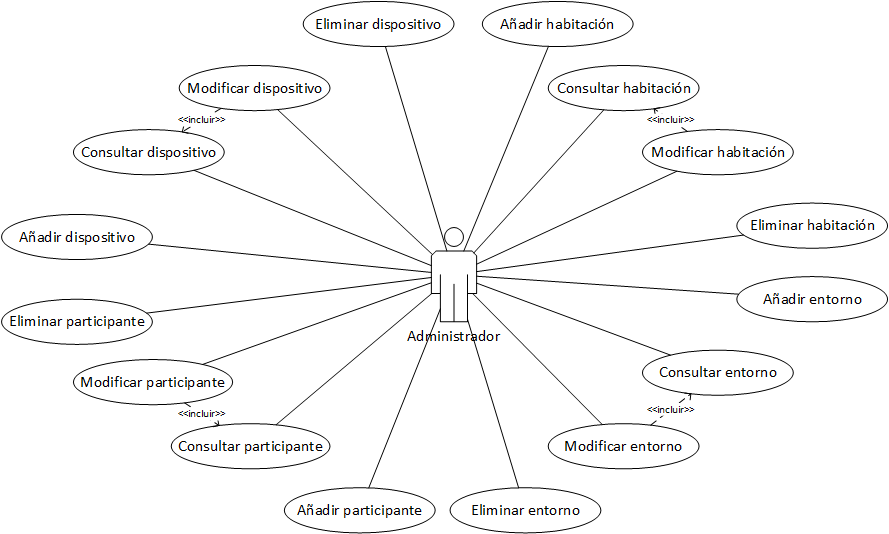
\includegraphics[width=0.7\textwidth]{4.Disenio/Imagenes/CU-Admin}
	\caption{Casos de uso del administrador.}
	\label{fig:cuAdmin}
\end{figure}


\subsection{Casos de uso en detalle}
Debido a la gran cantidad de casos de uso que hemos analizado en el sistema, la informaci\'on detallada de cada uno de los casos de uso est\'an localizados en el documento de \textit{Casos de uso} o conocido como \textit{Vista de escenarios}.
\section{Comprensi\'on de los casos de uso}
(actores: tipo usuario puede llevar a la confusion.)